\section{Model}

\subsection{Background}
% \noindent{\textbf{CDM based on RNN:}}
Firstly, we introduce RNN as an eventwise modeling method in cascade dynamics
modeling. A cascade $S=\{x_i|x_i=(t_i, u_i), u_i\in U \text{~and~}
t_i\in R^+\}_{i=1}^N$ is a set of propagations asendingly ordered by time,
where $U$ refers to all possible users in cascades. The $i$-th propagation $x_i$
is recorded as a tuple $(t_i, u_i)$ referring to activated time and activated user
respectively. At each step $k$, the $k$-th propagation are fed into hidden
units by nonlinear transformation $f$, jointly with the outputs from the
previous hidden units, updating the hidden state $h_k=f(x_i,h_{k-1})$. The
representation of hidden state $h_k$ can be considered as event embedding to
the $k$-th propagation~\cite{DuKDD2016}, and the output is trained to predict
the next propagation $x_{k+1}$ given $h_k$. In other words, we use RNN to
maximize the likelihood probability of observed propagations,
\begin{equation}
\label{eq:likelihood}
p(\textbf{x})=\prod_{k=1}^N p(x_{k+1}|h_k)
\end{equation}
% The embeddings of propagations $E(x_i)$ are given as inputs
% to RNN. At each step $k$, the network updates its hidden state $h_k=f(E(x_i),
% h_{k-1})$, where $f$ is certain nonlinear functions.  
% In RNN, the input to an encoder is an activation sequence
% $S=\{x_i|x_i=(t_i, u_i)\}_{i=1}^N$ asendingly ordered by time. The activation
% $x_i$ is recorded as a tuple $(t_i, e_i)$ referring to activated time and activated
% user respectively. The embeddings of activation are given as inputs to RNN. At
% each step $k$, the network updates 
% The current inputs are fed
% into hidden units by nonlinear transformation, jointly with the outputs from the
% previous hidden units, and then generate the next activation in cascade. The
% representation of hidden units can be recognized as the event embedding
% to the corresponding inputs. 
Based on sufficient observed cascades, RNN
can find an optimal solution for Eq.~(\ref{eq:likelihood})
in a huge functional space, avoiding the limits of prior knowledge. Thus, RNN
can be a promising method to capture the complex propagation patterns in cascade
dynamics modeling. 

However, RNN suffers crossing dependency problem caused by tree structure
propagations in cascade, shown in Fig.~\ref{fig:mot}. One of the possible
solutions is to construct a pooling layer above the hidden
units in order to build the direct dependency between the generation of $k$-th
propagation and all previous event embeddings, i.e.,
$p(x_{k+1} | \text{pooling}(h_1,\ldots,h_k))$. The simplest way of pooling can
be formalized as
\begin{equation}
\label{eq:pooling_frame}
s_k=\sum_{i=1}^k \alpha_{k,i} h_i \text{,~~~~~s.t.~} \sum_{i=1}^k
\alpha_{k,i}=1,
\end{equation}
where the weight $\alpha_{k,i}$ refers to the proportion of dependency between
next propagation and the $i$-th event embedding. Mean pooling and max pooling
are two popular choices for setting weights which takes the mean or element-wise
max of all hidden states. However, these two methods still ignore the structure
information in cascades.
% Mean pooling and max pooling
% are two popular choices for setting weights which takes the mean or
% element-wise max of all hidden states. 
% In this way, the generation of next activation
% can depend on any historical embedding instead of transitive dependency.
Intuitively, the weights can be settled according to the cascade tree, yet we
can hardly observe the tree structure even given the social relationships. Next
we propose attention mechanism to implement the pooling layer. 

\subsection{CYAN-RNN}
Attention mechanism is orginally used in neural machine translation (NMT),
firstly proposed by Bahdanau et.al~\cite{bahdanau2014neural}. In the
senario of attention-based NMT, the target words are translated by the words in
source sequence and attention mechanism can automatically learn the alignment
between source words and target words~\cite{}.
% the words in source sequence need to be
% aligned to the words in target sequence. 
% Attention-based RNN can adaptively
% learn the alignment between source and target sequences. 
However, there are two
problems when applying attention mechanism in cascade dyanmics modeling: 1)
only one single sequence can be observed in a cascade; 2) the size of alignments
in attention mechanism need to be updated when the context $\{h_1,\ldots,h_k\}$
is growing along with the proceeding propagations.

\begin{figure}[t]
\centering
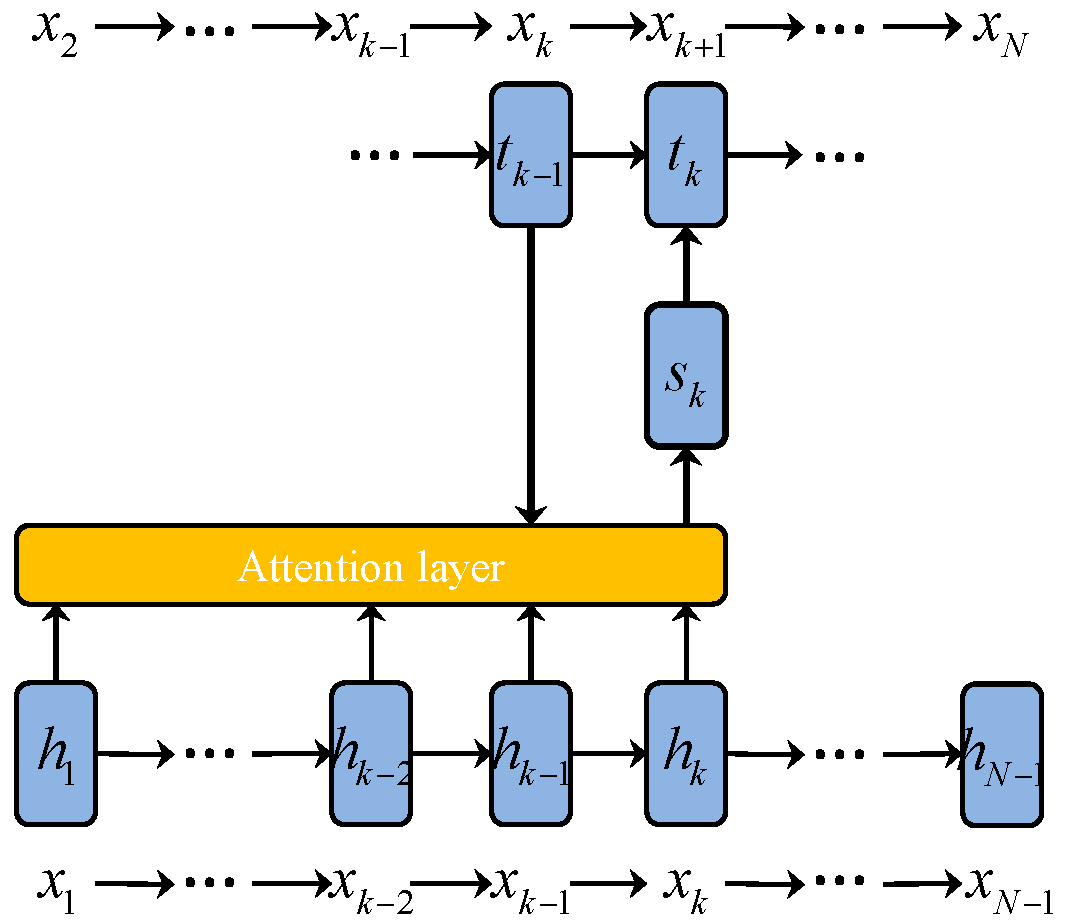
\includegraphics[width=0.35\textwidth]{figs/cyanrnn_framework.png}
\caption{The architecture of CYAN-RNN. The figure presents the case when
predicting the $(k+1)$-th propagation. The sequence in bottom is the observed
cascade and the sequence in top is the cascade shifted one step
according to the observation. The blue rectangles refer to representations from
the hidden units in source sequence, attention layer, and hidden units in
target sequence. The yellow rectangle is a component functioned in neural
network.}
\label{fig:cyrnn_frame}
\end{figure}

Thus, we propose CYAN-RNN for cascade dynamics modeling, applying a dynamic
attention mechanism to solve the crossing dependency problem. The architecture
of CYAN-RNN is shown in Fig.~\ref{fig:cyrnn_frame}. In CYAN-RNN, we conduct the
observed cascade as the source sequence. The target sequence is the copy of
source sequence, shifting one step of the copy backwards. The objective is to
jointly predict the next propagation and learn the alignment of dependency
between the next propagation and histories. 
% As to the target
% sequence, we copy the source sequence and then shift one step of the copy backwards. 
According to the architecture, we define each conditional probability in
Eq.~(\ref{eq:likelihood}) as:
\begin{equation}
\label{eq:cond_prob}
p(x_{k+1}|x_1,\ldots,x_k)=g(x_k, t_{k}, s_{k}),
\end{equation}
where $g$ is an objective function defined the joint probability of
propagation on activated user and activated time. Here we use the objective function
defined on RMTPP~\cite{DuKDD2016}.
% \begin{equation}
% \label{eq:rmtpp}
% \begin{aligned}
% g(x_k,t_{k},s_{k})&=p(u_{k+1}|t_k, s_k, x_k)\cdot p(t_{k+1}| t_k, s_k, x_k)\\
% &=\text{softmax}(t_k, s_k, x_k)\cdot
% \lambda(t_{k+1})\exp\left(-\int_{t_k}^{t_{k+1}}\lambda(\tau)d\tau \right)
% \end{aligned}
% \end{equation}
The $t_k$ is a hidden state related
to the $k$-th step of target sequence, computed by
\begin{equation}
\label{eq:target_embedding}
t_k = f(x_k, t_{k-1}, s_k),
\end{equation}
where 
% subscript in exponential function is the index of vector.   
$f$ is
a nonlinear activation function, which can be either a \textit{tanh} or
\textit{sigmoid} function. The context vector $s_k$ is calculated by
Eq.~(\ref{eq:pooling_frame}) where the weights $\alpha_{k,.}$ 
% in proposed attention mechanism 
is updated by the growth context
$\{h_1,\ldots,h_k\}$ and $t_{k-1}$. We can get the weights
\begin{equation}
\label{eq:alpha}
\alpha_{k,i}=\frac{\exp(e_{k,i})}{\sum_{j=1}^k \exp(e_{k,j})},
\end{equation}
where
\begin{equation}
\label{eq:score}
e_{k,i}=a(t_{k-1}, h_i)=v^T\tanh(W t_{k-1}+U h_i)
\end{equation}
scores how well the dependency between the $i$-th event
embedding and the output at the $k$-th step. The implementation of attention
mechanism in proposed model is briefly represented in Fig.~\ref{fig:att}. 

Given a collection of cascades $\mathcal{C}=\{S_m\}_{m=1}^M$, we suppose that
each cascade is independent on each other. As a result, the logarithmic
likelihood of a set of cascades is the sum of logarithmic likelihood of individual cascade.
In this way, the negative logarithmic likelihood of the set of cascades can be
estimated as
\begin{equation}
\mathcal{L}(\mathcal{C})=-\sum_{m=1}^M \sum_{k=1}^{N_m} \left[
g(x_k^{(m)}, t_{k}^{(m)}, s_{k}^{(m)}) \right], 
\end{equation}
and we can learn parameters of the proposed model by minimizing the negative
logarithmic likelihood.
%  $\arg \min_\theta \mathcal{L}(\mathcal{C})$, where $\theta$ is the
% parameter set in the model. 
With the attention mechanism, the alignment
weigts $\alpha_{k,.}$ can be directly updated through the cost function, thus
exploit an expected representation $s_k$ over all historic event embeddings for
each step $k$.

% The weights in proposed attention
% mechanism $s_k=\sum_{i=1}^k \alpha_i h_i$   
% The context vector $s_k$ is a representation, calculated in
% Eq.~(\ref{eq:pooling_frame}).

% to model cascade dynamics, the learned weights in
% attention and also infer the tree structure of propagations. The architecture of CYAN-RNN is shown in
% Fig.~\ref{fig:framework}.
% We firstly conduct the observed cascade as the source sequence.
% Then we copy the cascade and then shift one step of the copy backwards as the target
% sequence. 
 
\begin{figure}[ht!]
\centering
\subfigure[] {
\label{fig:att}
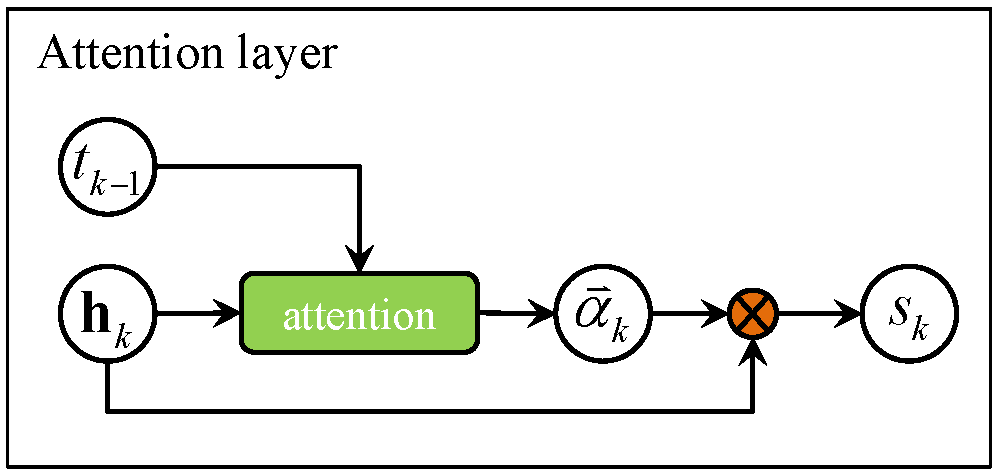
\includegraphics[width=0.35\textwidth]{figs/att.png}
}
\subfigure[] {
\label{fig:cov}
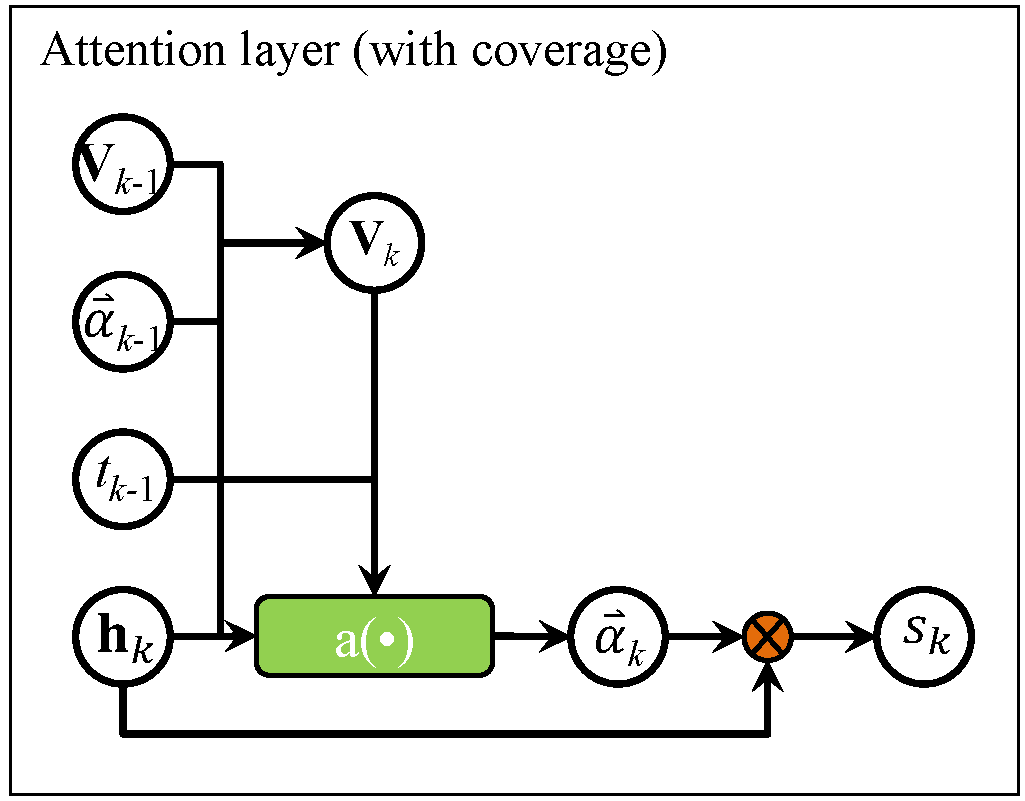
\includegraphics[width=0.35\textwidth]{figs/cov.png}
}
\caption{Two kinds of implementation on attention. (a) Attention mechanism
applied in CYAN-RNN; (b) Attention mechanism with coverage applied in CYAN-RNN
(cov). Note that $\textbf{h}_k=(h_1,\ldots,h_k)$ is matrix assembled by all
historic event embeddings at step $k$ and $\textbf{v}_k=(v_1,\ldots,v_k)$ is
a coverage martix containing all $k$-th coverage vectors.}
\end{figure}

\subsection{CYAN-RNN with Coverage}
\label{sec:coverage}

Although CYAN-RNN is proposed to better model cascade dynamics in consideration
of crossing dependency problem, the proposed model still suffer
\emph{over-dependent} and \emph{under-dependent} problems when applying
attention mechanism.
As the exmaple shown in Fig.~\ref{fig:mot}, if the user $u_1$ is an influential
user and his propagation is key to the cascade, the propagation activated by
$u_4$ may perfer to depend more on embedding of $(t_1, u_1)$ instead of $(t_2, u_2)$.
Here embedding of $(t_1, u_1)$ is over-dependent and embedding of $(t_2, u_2)$
is under-dependent. In practice, it is a common phenomenon that users may have a
higher probability activated by recent propagation than past ones~\cite{} and we
also conduct experiments to illustrate it (see section~\ref{sec:exp}).

The two problems are caused by memoryless of dynamic attention mechanism.
Inspired by linguistic coverage model~\cite{tu2016modeling}, we formulate the
general form of coverage, keeping historical alignments so
as to release the over-dependent and under-dependent problems. The $k$-th step
of coverage is defined as
\begin{equation}
\label{eq:cov}
V_{k,i}=f\left(V_{k-1, i}, \alpha_{k-1,i}, t_{k-1}, h_i\right).
\end{equation}
Remarkably, as the increasing propagations and alignments, $V_{k,k}$ and
$\alpha_{k,k}$ have no corresponding values in $V_{k-1,.}$ and
$\alpha_{k-1,.}$. Thus, we fill up with zeros in our works. 
Compared with $V_{k,i}$, $V_{k-1,i}$ 
At each step $k$, the $k$-th coverage serves an additional input to the
attention mechanism, providing complementary information of that how about the
dependencies of historical event embeddings are in the past. The rewritten
alignment calculation in Eq.~(\ref{eq:score}) by coverage can be
formalized~\footnote{The formalization is determined by the incremental length
of alignment weights. If we use the last coverage $V_{k-1,.}$ instead of
$V_{k,.}$ (like~\cite{tu2016modeling}) to update $e_{k,.}$ at each $k$
step, we will lose certain coverage information and cause unbalance
calculation about $k$-th event embedding, proved by our preliminary experiments.} as
\begin{equation}
\label{eq:att_cov}
\begin{aligned}
e_{k,i} &= a(t_{k-1}, h_i, V_{k,i}) \\
& = v^T\tanh(W t_{k-1}+U h_i+Z V_{k,i}).
\end{aligned}
\end{equation}
We expect that the alignment weights would be focus more on recent event
embeddings. The expectation will be validated in section~\ref{sec:exp}.   

\subsection{Window Size}
Practically, a cascade may last long and the propagation length would be huge,
causing an extreme computation cost when applying dynamic attention mechanism
proposed in CYAN-RNN. According to perference of users interests on recent
propagations, we consider a hyper-parameter, symboled by \emph{window size}
$l$, limiting the size of alignments so that the predicted task would only depend on
last $l$ propagations. Empirically, we set $l=200$ in most cases.

% Thus, the attention mechanism only need to calculate the
% $\max (k, t)$ historical event embeddings 
